\documentclass[14pt]{extarticle}
\usepackage{amssymb,amsthm,amsmath, color}
\usepackage{graphicx}
\usepackage{float}
\usepackage{fullpage}
\usepackage{subfigure}
\usepackage{graphics}

\newtheorem{theorem}{Theorem}[section]
\newtheorem{lemma}[theorem]{Lemma}
\newtheorem{proposition}[theorem]{Proposition}
\newtheorem{claim}[theorem]{Claim}
\newtheorem{corollary}[theorem]{Corollary}
\newtheorem{definition}[theorem]{Definition}
\newtheorem{observation}[theorem]{Observation}
\newtheorem{fact}[theorem]{Fact}
\newtheorem{property}{Property}
\newtheorem{remark}{Remark}[section]
\newtheorem{notation}{Notation}[section]
\newtheorem{example}{Example}[section]
\newtheorem{algorithm}{Algorithm}
\newtheorem{conjecture}{Conjecture}
\newtheorem{question}[conjecture]{Question}

\begin{document}
\textbf{CSE 2321 Homework 3}

\textbf{Turn In:} Submit to the Carmen dropbox a PDF file generated from LaTex source (see the template file provided with this homework and the Piazza post on LaTex).

\textbf{Reminder:} Homework should be worked on individually. If you are stuck on a problem, please spend time thinking about the problem and trying different approaches before seeking help in office hours. If you come to office hours you will benefit more if you have already attempted these problems. 

\begin{enumerate}

\item (5 pts) Let $A = \{1, 2, 3, 6\}$ and $B = \{2, 3, 5, 6\}$.\\Let $S$ be a set, and $Pow(S)$ be the power set of $S$.
\begin{enumerate}
\item What is $|Pow(A)|$?
\item List the elements of $Pow(A)$.
\item What is $|Pow(A \cup B)|$?
\item What is $|Pow(A \cap B)|$?
\item List the elements of $Pow(A \setminus B)$.
\end{enumerate}

\item (10 pts) Let $\mathbb{N}$ be the set of natural numbers (including 0). Define the following sets using set builder notation. You should do this in a way that is entirely mathematical, contains no words, and does not rely on recognizing a pattern. \\For example, if asked to define ``The set of natural numbers divisible by 3'' then 
\\$\{x \in \mathbb{N} : \mbox{x is divisible by 3}\}$ or $\{0, 3, 6, \ldots\}$ would not be accepted\\
$\{x \in \mathbb{N} : \exists y \in \mathbb{N}, x \div 3 = y \}$ would be accepted
\begin{enumerate}
\item The set of even numbers.
\item The set of prime numbers. Recall that 2 is the smallest prime.
\end{enumerate}

\item (10 pts) Define sets $A, B, X, Y, Z$ (i.e.~give a specific example) which demonstrate that:
\begin{enumerate}
\item $B \cup A \neq (A \setminus B) \cup (B \setminus A)$.
\item $Z \setminus (X \cup Y) \neq (Z \cap X) \cup (Z \cap Y)$.
\end{enumerate}

\item (10 pts) We say a graph $G = (V, E)$ is \textit{bipartite} if there are sets $V_1 \subseteq V$ and $V_2 \subseteq V$ such that \textbf{all} of the following conditions hold:
\begin{itemize}
\item $V_1 \cap V_2 = \emptyset$
\item $V_1 \cup V_2 = V$
\item $\forall \{u, v\} \in E$, $\left[(u \in V_1 \land v \in V_2) \lor (v \in V_1 \land u \in V_2)\right]$
\end{itemize}
Show that the following graph is bipartite by finding $V_1$ and $V_2$ which meet these conditions. Redraw the graph so that $V_1$ is on the left and $V_2$ on the right.
\begin{figure}[H]
	\centering
  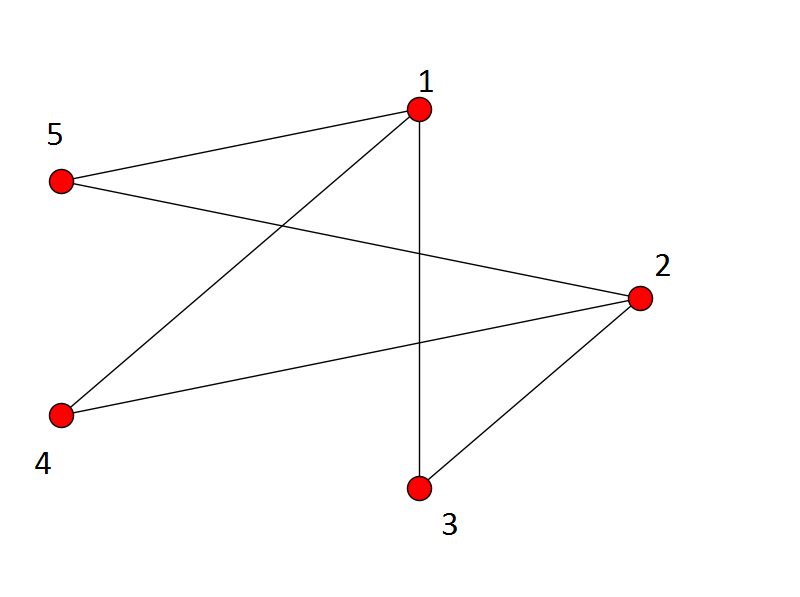
\includegraphics[width=0.5\textwidth]{figure_2.png}
\end{figure}

\item (5 pts) Find an Eulerian cycle in this graph and list the vertices in the order visited by the cycle:
\begin{figure}[H]
	\centering
  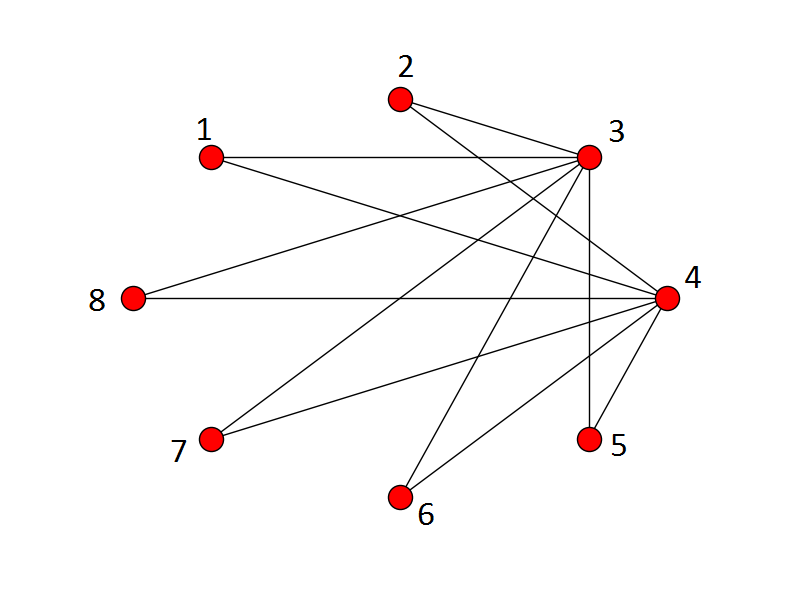
\includegraphics[width=0.5\textwidth]{figure_1.png}
\end{figure}

\item (10 pts) Using the proof techniques and format guidelines presented in lecture, prove that for all $n \geq 1$ the following is true:
\[
\sum_{i=1}^{n} \frac{1}{i(i+1)} = \frac{n}{n+1}.
\]
Hint: use the induction proof that $\sum_{i=1}^{n} i = \frac{n(n+1)}{2}$ as a guide.

\end{enumerate}



\end{document}
